

\section*{ID: beca03de}
A rectangle has a length that is 15 times its width. The function $y=(15 w)(w)$ represents this situation, where $y$ is the area, in square feet, of the rectangle and $y>0$. Which of the following is the best interpretation of $15 w$ in this context?\\
A. The length of the rectangle, in feet\\
B. The area of the rectangle, in square feet\\
C. The difference between the length and the width of the rectangle, in feet\\
D. The width of the rectangle, in feet

\section*{ID: 91e7ea5e}
$$
h(x)=2(x-4)^{2}-32
$$

The quadratic function $h$ is defined as shown. In the $x y$-plane, the graph of $y=h(x)$ intersects the $x$-axis at the points $(0,0)$ and $(t, 0)$, where $t$ is a constant.

What is the value of $t$ ?\\
A. 1\\
B. 2\\
C. 4\\
D. 8

\section*{ID: 8490cc45}
The function $f$ is defined by $f(x)=(-8)(2)^{x}+22$. What is the $y$-intercept of the graph of $y=f(x)$ in the $x y$-plane?\\
A. $(0,14)$\\
B. $(0,2)$\\
C. $(0,22)$\\
D. $(0,-8)$\\
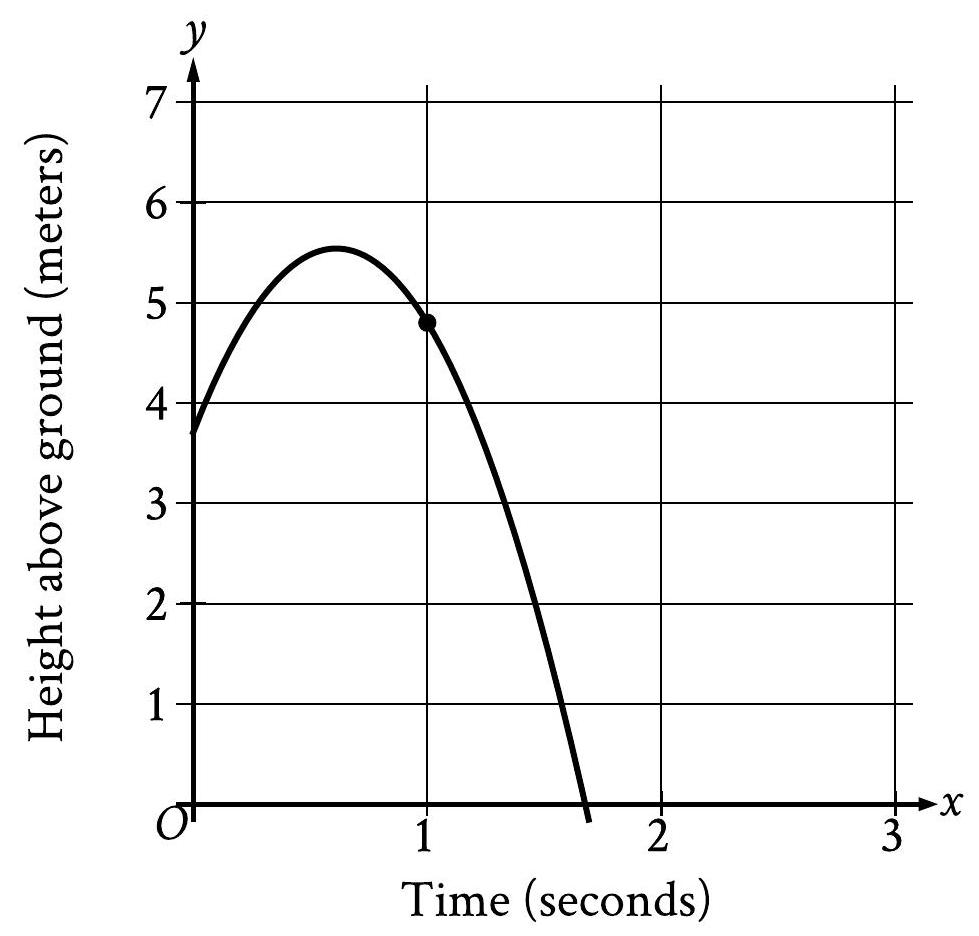
\includegraphics[max width=\textwidth, center]{2025_06_15_5ccb8dd1752fe76599e7g-004}

The graph shows the height above ground, in meters, of a ball $x$ seconds after the ball was launched upward from a platform. Which statement is the best interpretation of the marked point (1.0, 4.8) in this context?\\
A. 1.0 second after being launched, the ball's height above ground is 4.8 meters.\\
B. 4.8 seconds after being launched, the ball's height above ground is 1.0 meter.\\
C. The ball was launched from an initial height of 1.0 meter with an initial velocity of 4.8 meters per second.\\
D. The ball was launched from an initial height of 4.8 meters with an initial velocity of 1.0 meter per second.

$$
f(x)=9,000(0.66)^{x}
$$

The given function $f$ models the number of advertisements a company sent to its clients each year, where $x$ represents the number of years since 1997 , and $0 \leq x \leq 5$. If $y=f(x)$ is graphed in the $x y$-plane, which of the following is the best interpretation of the $y$-intercept of the graph in this context?\\
A. The minimum estimated number of advertisements the company sent to its clients during the 5 years was 1,708 .\\
B. The minimum estimated number of advertisements the company sent to its clients during the 5 years was 9,000 .\\
C. The estimated number of advertisements the company sent to its clients in 1997 was 1,708 .\\
D. The estimated number of advertisements the company sent to its clients in 1997 was 9,000 .

The first term of a sequence is 9 . Each term after the first is 4 times the preceding term. If $w$ represents the $n$th term of the sequence, which equation gives $w$ in terms of $n$ ?\\
A. $w=4\left(9^{n}\right)$\\
B. $w=4\left(9^{n-1}\right)$\\
C. $w=9\left(4^{n}\right)$\\
D. $w=9\left(4^{n-1}\right)$\\
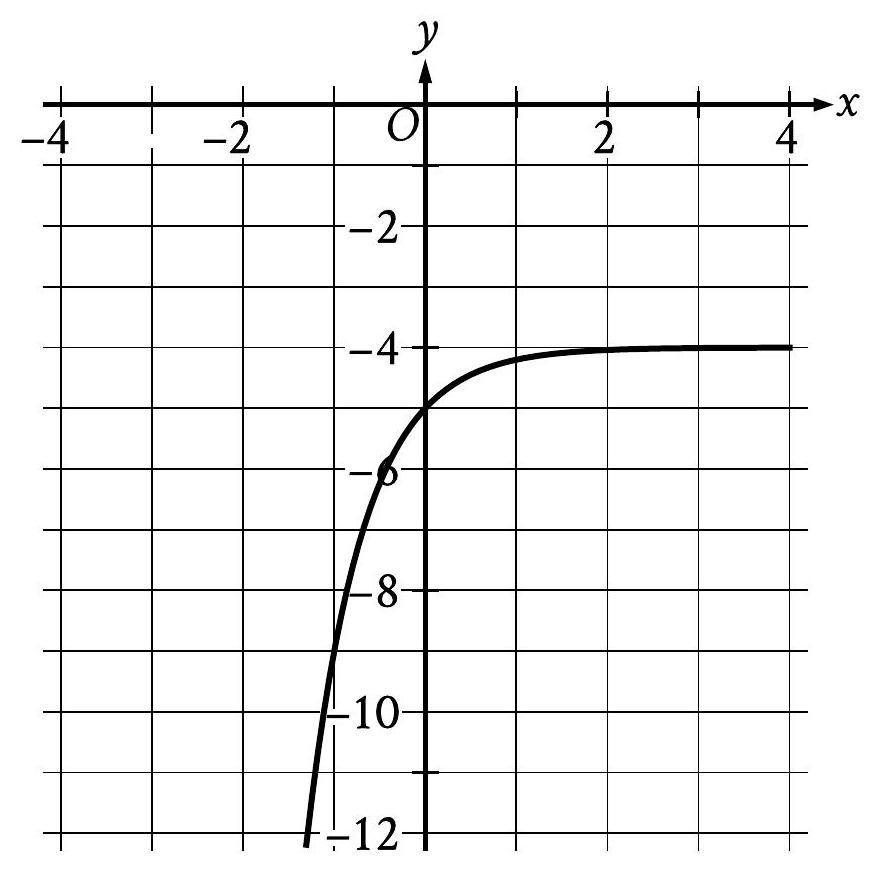
\includegraphics[max width=\textwidth, center]{2025_06_15_5ccb8dd1752fe76599e7g-007}

What is the $y$-intercept of the graph shown?\\
A. $(-1,-9)$\\
B. $(0,-5)$\\
C. $(0,-4)$\\
D. $(0,0)$

\begin{center}
\begin{tabular}{|l|l|}
\hline
Time (years) & Total amount (dollars) \\
\hline
0 & 604.00 \\
\hline
1 & 606.42 \\
\hline
2 & 608.84 \\
\hline
\end{tabular}
\end{center}

Rosa opened a savings account at a bank. The table shows the exponential relationship between the time $t$, in years, since Rosa opened the account and the total amount $n$, in dollars, in the account. If Rosa made no additional deposits or withdrawals, which of the following equations best represents the relationship between $t$ and $n$ ?\\
A. $n=$ msup\\
B. $n=$ msup\\
C. $n=604 \mathrm{msup}$\\
D. $n=0.004 \mathrm{msup}$

\section*{ID: b8f13a3a}
Function $f$ is defined by $f(x)=-a^{x}+b$, where $a$ and $b$ are constants. In the $x y$-plane, the graph of $y=f(x)-12$ has a $y$ intercept at $\left(0,-\frac{75}{7}\right)$. The product of $a$ and $b$ is $\frac{320}{7}$. What is the value of $a$ ?

\section*{ID: 1ee962ec}
\begin{center}
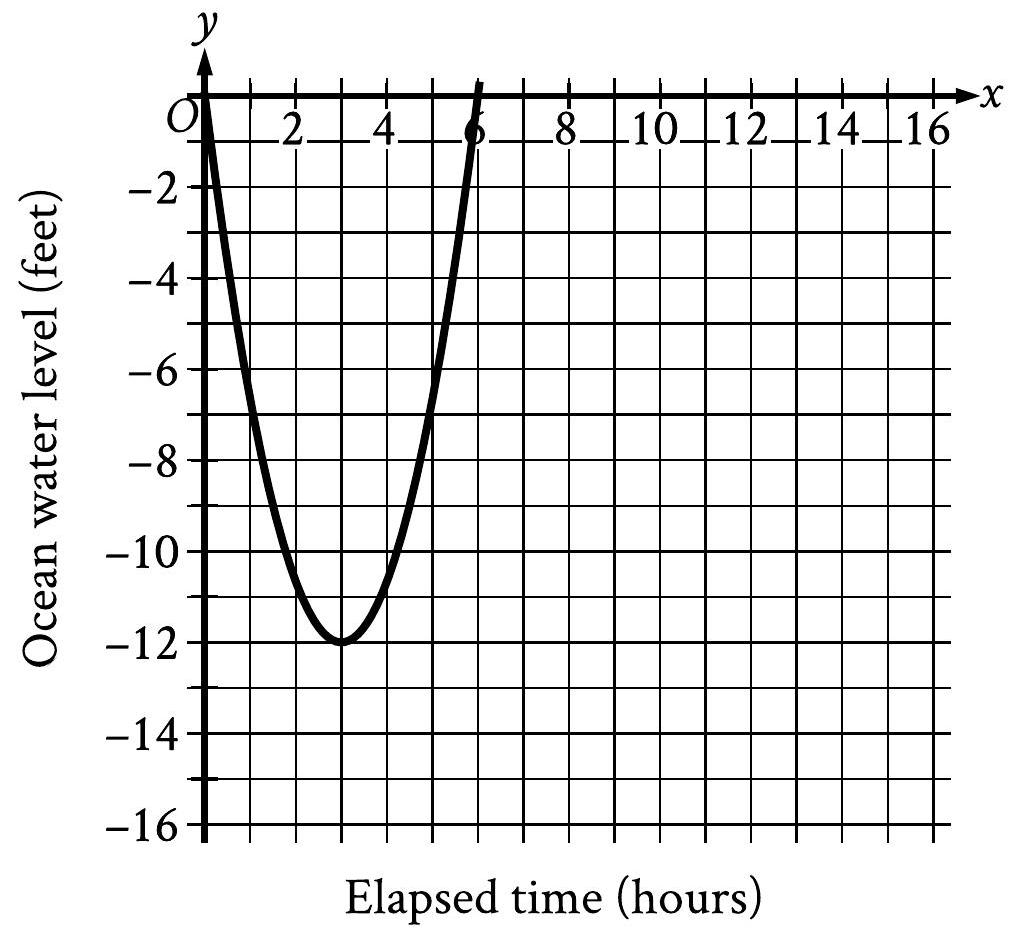
\includegraphics[max width=\textwidth]{2025_06_15_5ccb8dd1752fe76599e7g-010}
\end{center}

Scientists recorded data about the ocean water levels at a certain location over a period of 6 hours. The graph shown models the data, where $y=0$ represents sea level. Which table gives values of $x$ and their corresponding values of $y$ based on the model?\\
A.

\begin{center}
\begin{tabular}{|c|c|}
\hline
$x$ & $y$ \\
\hline
0 & -12 \\
\hline
0 & 3 \\
\hline
3 & 6 \\
\hline
\end{tabular}
\end{center}

B.

\begin{center}
\begin{tabular}{|c|c|}
\hline
$x$ & $y$ \\
\hline
0 & 0 \\
\hline
3 & 12 \\
\hline
0 & -6 \\
\hline
\end{tabular}
\end{center}

c.

\begin{center}
\begin{tabular}{|c|c|}
\hline
$x$ & $y$ \\
\hline
0 & 0 \\
\hline
3 & -12 \\
\hline
6 & 0 \\
\hline
\end{tabular}
\end{center}

D.

\begin{center}
\begin{tabular}{|l|l|}
\hline
$x$ & $y$ \\
\hline
0 & 0 \\
\hline
\end{tabular}
\end{center}

The function $f$ is defined by $f(x)=4+\sqrt{x}$. What is the value of $f(144)$ ?\\
A. 0\\
B. 16\\
C. 40\\
D. 76

\section*{ID: f89af023}
A rectangular volleyball court has an area of 162 square meters. If the length of the court is twice the width, what is the width of the court, in meters?\\
A. 9\\
B. 18\\
C. 27\\
D. 54

\section*{ID: 7902bed0}
A machine launches a softball from ground level. The softball reaches a maximum height of 51.84 meters above the ground at 1.8 seconds and hits the ground at 3.6 seconds. Which equation represents the height above ground $h$, in meters, of the softball $t$ seconds after it is launched?\\
A. $h=-t^{2}+3.6$\\
B. $h=-t^{2}+51.84$\\
C. $h=-16 \mathrm{msup}-3.6$\\
D. $h=-16 \mathrm{msup}+51.84$

The function $f$ is defined by $f(x)=a^{x}+b$, where $a$ and $b$ are constants. In the $x y$-plane, the graph of $y=f(x)$ has an $x$ intercept at $(2,0)$ and a $y$-intercept at $(0,-323)$. What is the value of $b$ ?

\section*{ID: e53add44}
$S(n)=38,000 a^{n}$

The function $S$ above models the annual salary, in dollars, of an employee $n$ years after starting a job, where $a$ is a constant. If the employee's salary increases by $4 \%$ each year, what is the value of $a$ ?\\
A. 0.04\\
B. 0.4\\
C. 1.04\\
D. 1.4

\section*{ID: 9654add7}
$f(x)=-500 x^{2}+25,000 x$\\
The revenue $f(x)$, in dollars, that a company receives from sales of a product is given by the function $f$ above, where $x$ is the unit price, in dollars, of the product. The graph of $y=f(x)$ in the $x y$-plane intersects the $x$-axis at 0 and $a$. What does $a$ represent?\\
A. The revenue, in dollars, when the unit price of the product is \$0\\
B. The unit price, in dollars, of the product that will result in maximum revenue\\
C. The unit price, in dollars, of the product that will result in a revenue of \$0\\
D. The maximum revenue, in dollars, that the company can make

\section*{ID: 263f9937}
Growth of a Culture of Bacteria

\begin{center}
\begin{tabular}{|c|c|}
\hline
Day & \begin{tabular}{c}
Number of bacteria per \\
milliliter at end of day \\
\end{tabular} \\
\hline
1 & $2.5 \times 10^{5}$ \\
\hline
2 & $5.0 \times 10^{5}$ \\
\hline
3 & $1.0 \times 10^{6}$ \\
\hline
\end{tabular}
\end{center}

A culture of bacteria is growing at an exponential rate, as shown in the table above.\\
At this rate, on which day would the number of bacteria per milliliter reach\\
$5.12 \times 10^{8}$ ?\\
A. Day 5\\
B. Day 9\\
C. Day 11\\
D. Day 12

\section*{ID: 926c246b}
$D=5,640(1.9)^{t}$

The equation above estimates the global data traffic $D$, in terabytes, for the year that is $t$ years after 2010. What is the best interpretation of the number 5,640 in this context?\\
A. The estimated amount of increase of data traffic, in terabytes, each year\\
B. The estimated percent increase in the data traffic, in terabytes, each year\\
C. The estimated data traffic, in terabytes, for the year that is $t$ years after 2010\\
D. The estimated data traffic, in terabytes, in 2010

\section*{ID: 4dd4efcf}
$$
f(x)=a x^{2}+4 x+c
$$

In the given quadratic function, $a$ and $c$ are constants. The graph of $y=f(x)$ in the $x y$-plane is a parabola that opens upward and has a vertex at the point $(h, k)$, where $h$ and $k$ are constants. If $k<0$ and $f(-9)=f(3)$, which of the following must be true?\\
l. $c<0$\\
II. $a \geq 1$\\
A. I only\\
B. II only\\
C. I and II\\
D. Neither I nor II\\




















































The function $f$ is defined by $f(x)=\frac{1}{6 x}$. What is the value of $f(x)$ when $x=3$ ?\\
A. $\frac{1}{3}$\\
B. $\frac{1}{6}$\\
C. $\frac{1}{9}$\\
D. $\frac{1}{18}$








\section*{ID: a45ffacb}
Function $f$ is defined by $f(x)=-a^{x}+b$, where $a$ and $b$ are constants. 
In the $x y$-plane, the graph of $y=f(x)-15$ has a $y$ intercept at 
$\left(0,-\frac{99}{7}\right)$. The product of $a$ and $b$ is $\frac{65}{7}$. 
What is the value of $a$ ?

$$
g(x)=x^{2}+55
$$

What is the minimum value of the given function?\\
A. 0\\
B. 55\\
C. 110\\
D. 3,025












$$
f(x)=(x-14)(x+19)
$$

The function $f$ is defined by the given equation. For what value of $x$ does $f(x)$ reach its minimum?\\
A. -266\\
B. -19\\
C. $-\frac{33}{2}$\\
D. $-\frac{5}{2}$\\
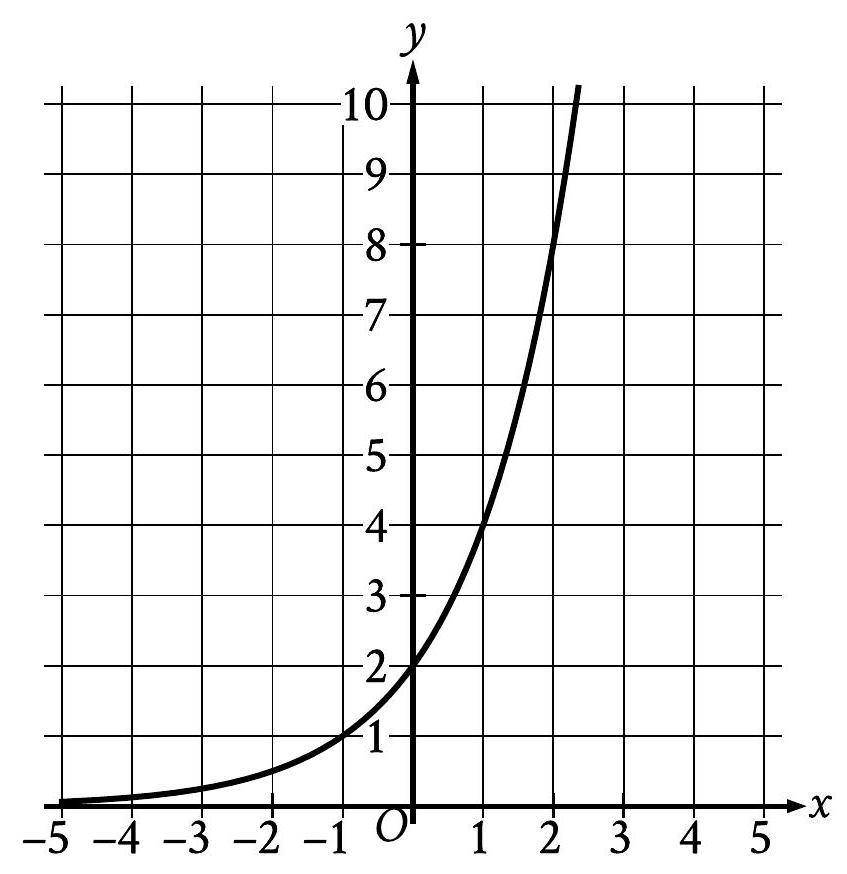
\includegraphics[max width=\textwidth, center]{2025_06_15_5ccb8dd1752fe76599e7g-035}

What is the $y$-intercept of the graph shown?\\
A. $(0,0)$\\
B. $(0,2)$\\
C. $(2,0)$\\
D. $(2,2)$\\
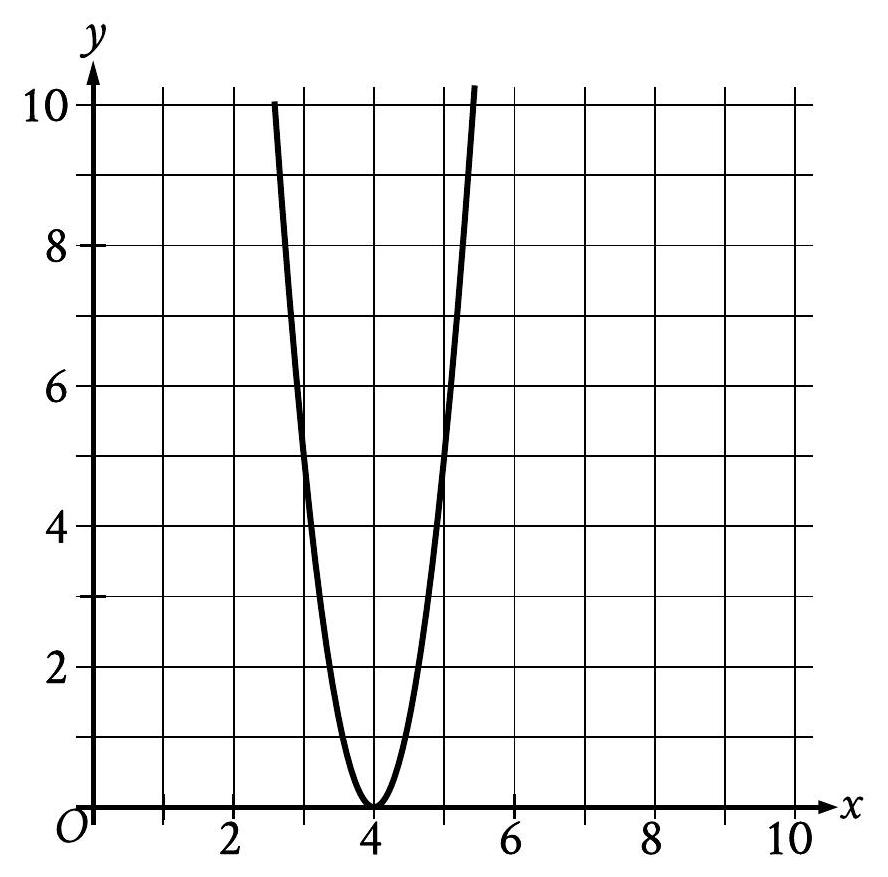
\includegraphics[max width=\textwidth, center]{2025_06_15_5ccb8dd1752fe76599e7g-036}

What is the $x$-intercept of the graph shown?\\
A. $(-5,0)$\\
B. $(5,0)$\\
C. $(-4,0)$\\
D. $(4,0)$

$$
f(x)=(x+6)(x-4)
$$

If the given function $f$ is graphed in the $x y$-plane, where $y=f(x)$, what is the $x$-coordinate of an $x$-intercept of the graph?

\section*{ID: be0c419e}
Immanuel purchased a certain rare coin on January 1. The function $f(x)=65(1.03)^{x}$, where $0 \leq x \leq 10$, gives the predicted value, in dollars, of the rare coin $x$ years after Immanuel purchased it. What is the best interpretation of the statement " $f(8)$ is approximately equal to $82^{\prime \prime}$ in this context?\\
A. When the rare coin's predicted value is approximately 82 dollars, it is $8 \%$ greater than the predicted value, in dollars, on January 1 of the previous year.\\
B. When the rare coin's predicted value is approximately 82 dollars, it is 8 times the predicted value, in dollars, on January 1 of the previous year.\\
C. From the day Immanuel purchased the rare coin to 8 years after Immanuel purchased the coin, its predicted value increased by a total of approximately 82 dollars.\\
D. 8 years after Immanuel purchased the rare coin, its predicted value is approximately 82 dollars.

\section*{ID: ce579859}
A model estimates that at the end of each year from 2015 to 2020, the number of squirrels in a population was $150 \%$ more than the number of squirrels in the population at the end of the previous year. The model estimates that at the end of 2016, there were 180 squirrels in the population. Which of the following equations represents this model, where $n$ is the estimated number of squirrels in the population $t$ years after the end of 2015 and $t \leq 5$ ?\\
A. $n=72$ msup\\
B. $n=72 \mathrm{msup}$\\
C. $n=180 \mathrm{msup}$\\
D. $n=180 \mathrm{msup}$

\section*{ID: 2f51abc2}
$$
f(x)=|59-2 x|
$$

The function $f$ is defined by the given equation. For which of the following values of $k$ does $f(k)=3 k$ ?\\
A. $\frac{59}{5}$\\
B. $\frac{59}{2}$\\
C. $\frac{177}{5}$\\
D. 59

\section*{ID: a31417d1}
From 2005 through 2014, the number of music CDs sold in the United States declined each year by approximately $15 \%$ of the number sold the preceding year. In 2005, approximately 600 million CDs were sold in the United States. Of the following, which best models C, the number of millions of CDs sold in the United States, $t$ years after 2005?\\
A. $C=600(0.15)^{t}$\\
B. $C=600(0.85)^{t}$\\
c. $C=600(1.15)^{t}$\\
D. $C=600(1.85)^{t}$

\section*{ID: 9afe2370}
The population $P$ of a certain city $y$ years after the last census is modeled by the equation below, where $r$ is a constant and $P_{0}$ is the population when $y=0$.\\
$P=P_{0}(1+r)^{y}$

If during this time the population of the city decreases by a fixed percent each year, which of the following must be true?\\
A. $r<-1$\\
B. $-1<r<0$\\
C. $0<r<1$\\
D. $r>1$

\section*{ID: ad376f1a}
\begin{center}
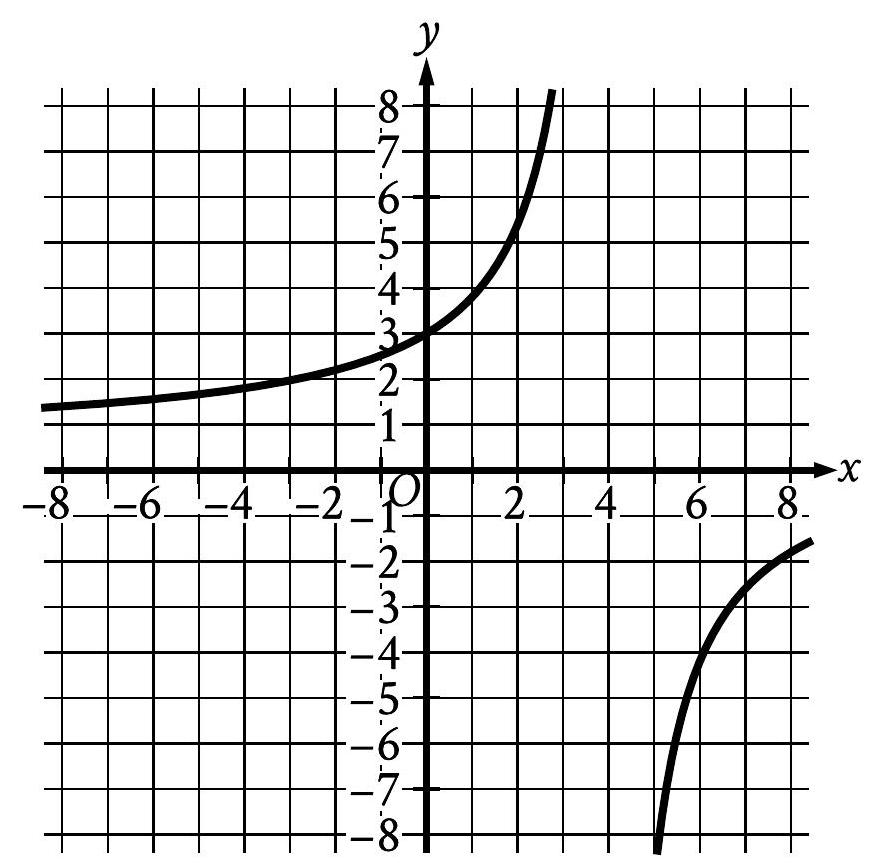
\includegraphics[max width=\textwidth]{2025_06_15_5ccb8dd1752fe76599e7g-043}
\end{center}

The graph of $y=f(x)$ is shown in the $x y$-plane. What is the value of $f(0)$ ?\\
A. -3\\
B. 0\\
C. $\frac{3}{5}$\\
D. 3\\
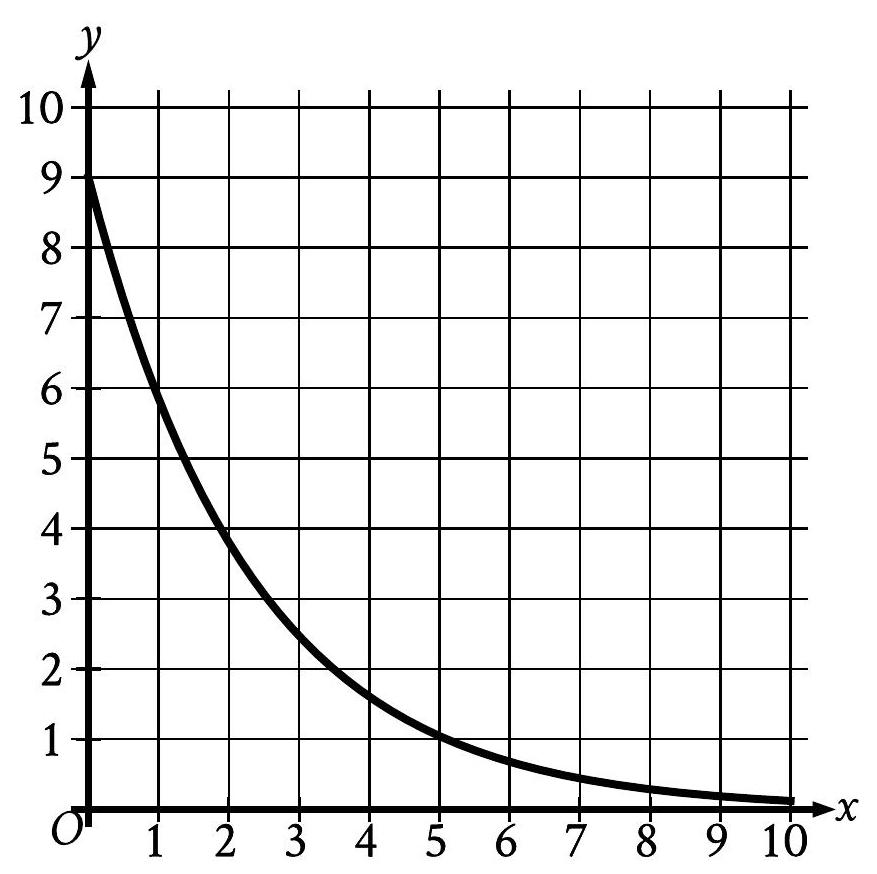
\includegraphics[max width=\textwidth, center]{2025_06_15_5ccb8dd1752fe76599e7g-044}

The graph gives the estimated number of catalogs $y$, in thousands, a company sent to its customers at the end of each year, where $x$ represents the number of years since the end of 1992 , where $0 \leq x \leq 10$. Which statement is the best interpretation of the $y$-intercept in this context?\\
A. The estimated total number of catalogs the company sent to its customers during the first 10 years was 9,000 .\\
B. The estimated total number of catalogs the company sent to its customers from the end of 1992 to the end of 2002 was 90.\\
C. The estimated number of catalogs the company sent to its customers at the end of 1992 was 9.\\
D. The estimated number of catalogs the company sent to its customers at the end of 1992 was 9,000 .

$$
f(x)=(x+6)(x+5)(x-4)
$$

The function $f$ is given. Which table of values represents $y=f(x)-3$ ?\\
A.

\begin{center}
\begin{tabular}{|c|c|}
\hline
$x$ & $y$ \\
\hline
-6 & -9 \\
\hline
-5 & -8 \\
\hline
4 & 1 \\
\hline
\end{tabular}
\end{center}

B.

\begin{center}
\begin{tabular}{|c|c|}
\hline
$x$ & $y$ \\
\hline
-6 & -3 \\
\hline
-5 & -3 \\
\hline
4 & -3 \\
\hline
\end{tabular}
\end{center}

c.

\begin{center}
\begin{tabular}{|c|c|}
\hline
$x$ & $y$ \\
\hline
-6 & -3 \\
\hline
-5 & -2 \\
\hline
4 & 7 \\
\hline
\end{tabular}
\end{center}

D.

\begin{center}
\begin{tabular}{|c|c|}
\hline
$x$ & $y$ \\
\hline
-6 & 3 \\
\hline
-5 & 3 \\
\hline
4 & 3 \\
\hline
\end{tabular}
\end{center}

The product of two positive integers is 546 . If the first integer is 11 greater than twice the second integer, what is the smaller of the two integers?\\
A. 7\\
B. 14\\
C. 39\\
D. 78

$$
f(x)=5,470(0.64)^{\frac{x}{12}}
$$

The function $f$ gives the value, in dollars, of a certain piece of equipment after $x$ months of use. If the value of the equipment decreases each year by $p \%$ of its value the preceding year, what is the value of $p$ ?\\
A. 4\\
B. 5\\
C. 36\\
D. 64

\section*{ID: c4cd5bcc}
In the $x y$-plane, the $y$-coordinate of the $y$-intercept of the graph of the function $f$ is c. Which of the following must be equal to $c$ ?\\
A. $f(0)$\\
B. $f(1)$\\
C. $f(2)$\\
D. $f(3)$

\section*{ID: 735a0a00}
$$
y=0.25 x^{2}-7.5 x+90.25
$$

The equation gives the estimated stock price $y$, in dollars, for a certain company $x$ days after a new product launched, where $0 \leq x \leq 20$. Which statement is the best interpretation of $(x, y)=(1,83)$ in this context?\\
A. The company's estimated stock price increased $\$ 83$ every day after the new product launched.\\
B. The company's estimated stock price increased $\$ 1$ every 83 days after the new product launched.\\
C. 1 day after the new product launched, the company's estimated stock price is $\$ 83$.\\
D. 83 days after the new product launched, the company's estimated stock price is $\$ 1$.

\section*{ID: 78d5f91a}
$$
f(x)=x^{3}+3 x^{2}-6 x-1
$$

For the function $f$ defined above, what is the value of $f(-1)$ ?\\
A. -11\\
B. -7\\
C. 7\\
D. 11\\
$y=4\left(2^{x}\right)$

Which of the following is the graph in the $x y$ plane of the given equation?\\
A.\\
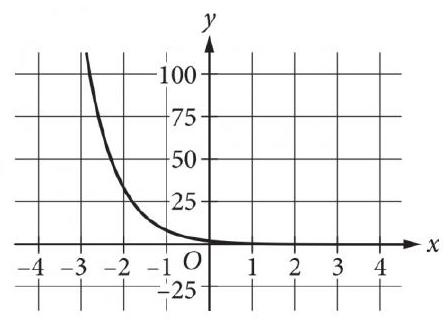
\includegraphics[max width=\textwidth, center]{2025_06_15_5ccb8dd1752fe76599e7g-051(1)}\\
B.\\
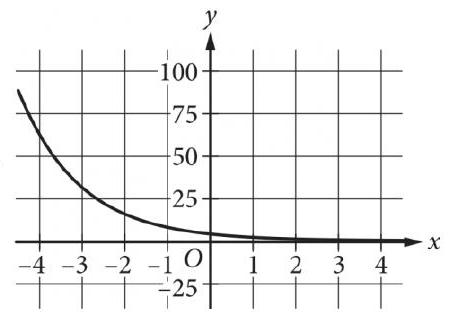
\includegraphics[max width=\textwidth, center]{2025_06_15_5ccb8dd1752fe76599e7g-051(3)}\\
C.\\
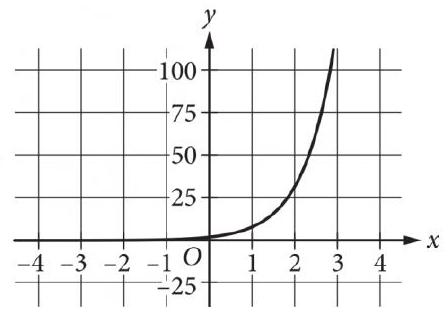
\includegraphics[max width=\textwidth, center]{2025_06_15_5ccb8dd1752fe76599e7g-051(2)}\\
D.\\
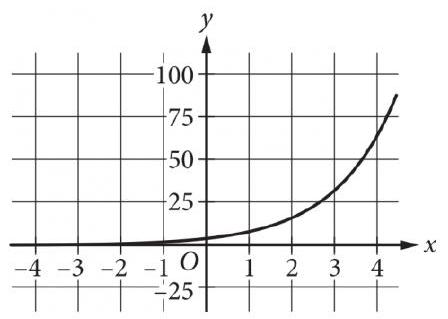
\includegraphics[max width=\textwidth, center]{2025_06_15_5ccb8dd1752fe76599e7g-051}

If $f(x)=\frac{x^{2}-6 x+3}{x-1}$\\
what is $f(-1)$ ?\\
A. -5\\
B. -2\\
C. 2\\
D. 5

\section*{ID: f2d60b99}
The function $f(x)=\frac{1}{9}(x-7)^{2}+3$ gives a metal ball's height above the ground $f(x)$, in inches, $x$ seconds after it started moving on a track, where $0 \leq x \leq 10$. Which of the following is the best interpretation of the vertex of the graph of $y=f(x)$ in the $x y$-plane?\\
A. The metal ball's minimum height was 3 inches above the ground.\\
B. The metal ball's minimum height was 7 inches above the ground.\\
C. The metal ball's height was 3 inches above the ground when it started moving.\\
D. The metal ball's height was 7 inches above the ground when it started moving.

The function $f(w)=6 w^{2}$ gives the area of a rectangle, in square feet $\left(\mathrm{ft}^{2}\right)$, if its width is $w \mathrm{ft}$ and its length is 6 times its width. Which of the following is the best interpretation of $f(14)=1,176$ ?\\
A. If the width of the rectangle is 14 ft , then the area of the rectangle is $1,176 \mathrm{ft}^{2}$.\\
B. If the width of the rectangle is 14 ft , then the length of the rectangle is $1,176 \mathrm{ft}$.\\
C. If the width of the rectangle is $1,176 \mathrm{ft}$, then the length of the rectangle is 14 ft .\\
D. If the width of the rectangle is $1,176 \mathrm{ft}$, then the area of the rectangle is $14 \mathrm{ft}^{2}$.

\begin{center}
\begin{tabular}{|c|c|}
\hline
$x$ & $f(x)$ \\
\hline
-1 & 10 \\
\hline
0 & 14 \\
\hline
1 & 20 \\
\hline
\end{tabular}
\end{center}

For the quadratic function $f$, the table shows three values of $x$ and their corresponding values of $f(x)$. Which equation defines $f$ ?\\
A. $f(x)=3 x^{2}+3 x+14$\\
B. $f(x)=5 x^{2}+x+14$\\
C. $f(x)=9 x^{2}-x+14$\\
D. $f(x)=x^{2}+5 x+14$

$$
f(t)=8,000(0.65)^{t}
$$

The given function $f$ models the number of coupons a company sent to their customers at the end of each year, where $t$ represents the number of years since the end of 1998 , and $0 \leq t \leq 5$. If $y=f(t)$ is graphed in the ty-plane, which of the following is the best interpretation of the $y$-intercept of the graph in this context?\\
A. The minimum estimated number of coupons the company sent to their customers during the 5 years was 1,428 .\\
B. The minimum estimated number of coupons the company sent to their customers during the 5 years was 8,000 .\\
C. The estimated number of coupons the company sent to their customers at the end of 1998 was 1,428 .\\
D. The estimated number of coupons the company sent to their customers at the end of 1998 was 8,000 .\\
$f(x)=2\left(3^{x}\right)$

For the function $f$ defined above, what is the value of $f(2)$ ?\\
A. 9\\
B. 12\\
C. 18\\
D. 36

An object's kinetic energy, in joules, is equal to the product of one-half the object's mass, in kilograms, and the square of the object's speed, in meters per second. What is the speed, in meters per second, of an object with a mass of 4 kilograms and kinetic energy of 18 joules?\\
A. 3\\
B. 6\\
C. 9\\
D. 36

\section*{ID: 92f812bb}
In the $x y$-plane, a parabola has vertex $(9,-14)$ and intersects the $x$-axis at two points. If the equation of the parabola is written in the form $y=a x^{2}+b x+c$, where $a$, $b$, and $c$ are constants, which of the following could be the value of $a+b+c$ ?\\
A. -23\\
B. -19\\
C. -14\\
D. -12\\
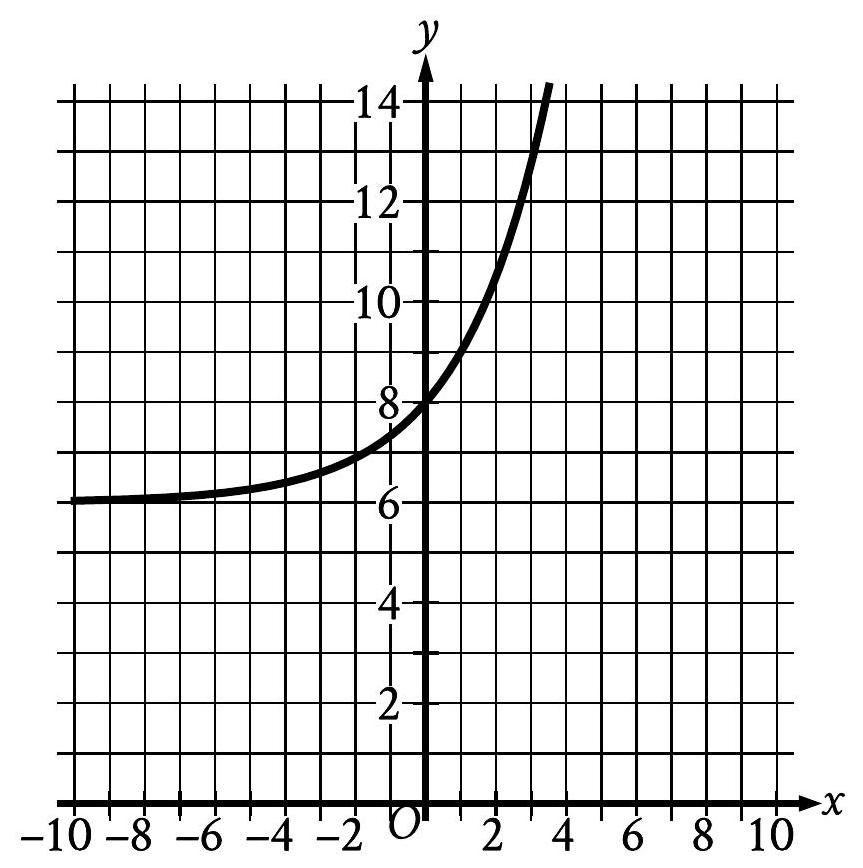
\includegraphics[max width=\textwidth, center]{2025_06_15_5ccb8dd1752fe76599e7g-060}

What is the $y$-intercept of the graph shown?\\
A. $(-8,0)$\\
B. $(-6,0)$\\
C. $(0,6)$\\
D. $(0,8)$

\begin{center}
\begin{tabular}{|c|c|}
\hline
$x$ & $p(x)$ \\
\hline
-2 & 5 \\
\hline
-1 & 0 \\
\hline
0 & -3 \\
\hline
1 & -1 \\
\hline
2 & 0 \\
\hline
\end{tabular}
\end{center}

The table above gives selected values of a polynomial function $p$. Based on the values in the table, which of the following must be a factor of $p$ ?\\
A. $(x-3)$\\
B. $(x+3)$\\
C. $(x-1)(x+2)$\\
D. $(x+1)(x-2)$

\section*{ID: 9da41c80}
A ball is dropped from an initial height of 22 feet and bounces off the ground repeatedly. The function $h$ estimates that the maximum height reached after each time the ball hits the ground is $85 \%$ of the maximum height reached after the previous time the ball hit the ground. Which equation defines $h$, where $h(n)$ is the estimated maximum height of the ball after it has hit the ground $n$ times and $n$ is a whole number greater than 1 and less than 10 ?\\
A. $h(n)=22(0.22)^{n}$\\
B. $h(n)=22(0.85)^{n}$\\
C. $h(n)=85$ msup\\
D. $h(n)=85(0.85)^{n}$\\
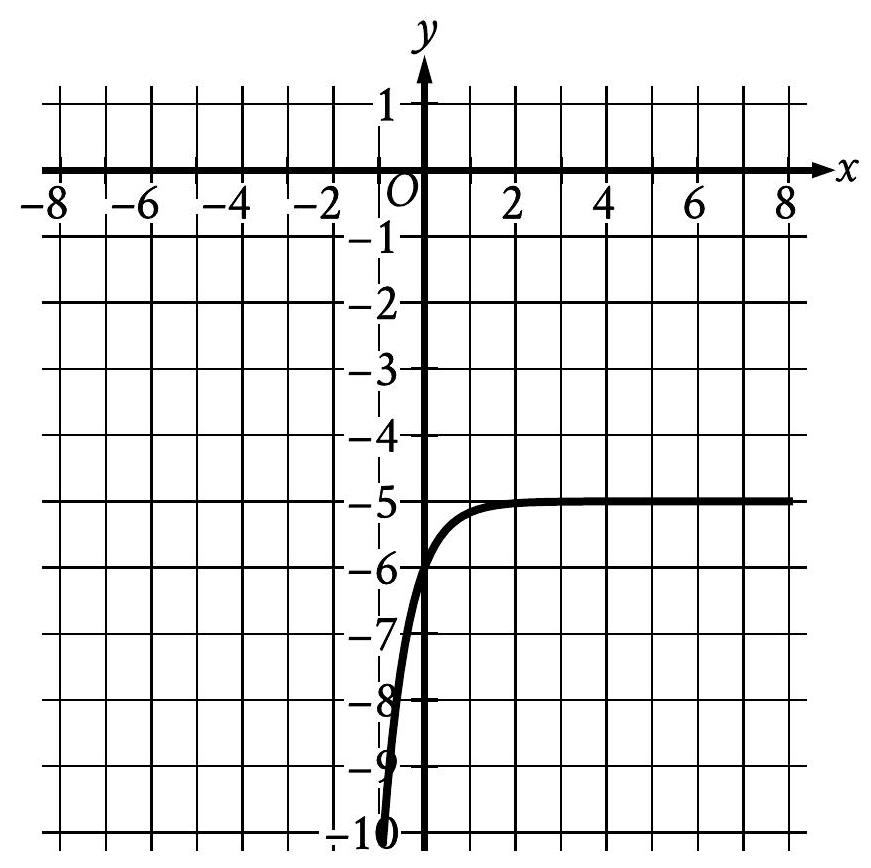
\includegraphics[max width=\textwidth, center]{2025_06_15_5ccb8dd1752fe76599e7g-063}

What is the $y$-intercept of the graph shown?\\
A. $(0,-6)$\\
B. $(-6,0)$\\
C. $(0,0)$\\
D. $(-5,-5)$

\section*{ID: d71f6dbf}
The height, in feet, of an object $x$ seconds after it is thrown straight up in the air can be modeled by the function $h(x)=-16 x^{2}+20 x+5$. Based on the model, which of the following statements best interprets the equation $h(1.4)=1.64$ ?\\
A. The height of the object 1.4 seconds after being thrown straight up in the air is 1.64 feet.\\
B. The height of the object 1.64 seconds after being thrown straight up in the air is 1.4 feet.\\
C. The height of the object 1.64 seconds after being thrown straight up in the air is approximately 1.4 times as great as its initial height.\\
D. The speed of the object 1.4 seconds after being thrown straight up in the air is approximately 1.64 feet per second.

The function $f$ is defined by $f(x)=x^{3}+9$. What is the value of $f(2)$ ?\\
A. 14\\
B. 15\\
C. 17\\
D. 18

\section*{ID: bba18ecb}
When the quadratic function $f$ is graphed in the $x y$-plane, where $y=f(x)$, its vertex is $(-3,6)$. One of the $x$-intercepts of this graph is $\left(-\frac{17}{4}, 0\right)$. What is the other $x$-intercept of the graph?\\
A. $\left(-\frac{29}{4}, 0\right)$\\
B. $\left(-\frac{7}{4}, 0\right)$\\
C. $\left(\frac{5}{4}, 0\right)$\\
D. $\left(\frac{17}{4}, 0\right)$

The function $f$ is defined by $f(x)=(x+3)(x+1)$. The graph of $f$ in the $x y$-plane is a parabola. Which of the following intervals contains the $x$-coordinate of the vertex of the graph of $f$ ?\\
A. $-4<x<-3$\\
B. $-3<x<1$\\
C. $1<x<3$\\
D. $3<x<4$

An engineer wanted to identify the best angle for a cooling fan in an engine in order to get the greatest airflow. The engineer discovered that the function above models the airflow $f(\theta)$, in cubic feet per minute, as a function of the angle of the fan $\boldsymbol{\theta}$, in degrees. According to the model, what angle, in degrees, gives the greatest airflow?\\
A. -0.28\\
B. 0.28\\
C. 27\\
D. 880

The function $f(t)=60,000(2)^{\frac{t}{410}}$ gives the number of bacteria in a population $t$ minutes after an initial observation. How much time, in minutes, does it take for the number of bacteria in the population to double?

\section*{ID: dd8ac009}
\begin{center}
\begin{tabular}{|l|l|}
\hline
Time (years) & Total amount (dollars) \\
\hline
0 & 670.00 \\
\hline
1 & 674.02 \\
\hline
2 & 678.06 \\
\hline
\end{tabular}
\end{center}

Sara opened a savings account at a bank. The table shows the exponential relationship between the time $t$, in years, since Sara opened the account and the total amount $d$, in dollars, in the account. If Sara made no additional deposits or withdrawals, which of the following equations best represents the relationship between $t$ and $d$ ?\\
A. $d=0.006$ msup\\
B. $d=670 \mathrm{msup}$\\
C. $d=$ msup\\
D. $d=$ msup

\section*{ID: 58dcc59f}
A landscaper is designing a rectangular garden. The length of the garden is to be 5 feet longer than the width. If the area of the garden will be 104 square feet, what will be the length, in feet, of the garden?

$$
P(t)=290(1.04)^{\left(\frac{4}{6}\right) t}
$$

The function $P$ models the population, in thousands, of a certain city $t$ years after 2005. According to the model, the population is predicted to increase by $n \%$ every 18 months. What is the value of $n$ ?\\
A. 0.38\\
B. 1.04\\
C. 4\\
D. 6

For the function $f, f(0)=86$, and for each increase in $x$ by 1 , the value of $f(x)$ decreases by $80 \%$. What is the value of $f(2)$ ?

\section*{ID: 59d1f4b5}
$$
M=1,800(1.02)^{t}
$$

The equation above models the number of members, $M$, of a gym $t$ years after the gym opens. Of the following, which equation models the number of members of the gym $q$ quarter years after the gym opens?\\
$M=1,800(1.02)^{\frac{q}{4}}$\\
A.\\
B. $M=1,800(1.02)^{4 q}$\\
C. $M=1,800(1.005)^{4 q}$\\
D. $M=1,800(1.082)^{q}$

\section*{ID: 281a4f3b}
A certain college had 3,000 students enrolled in 2015. The college predicts that after 2015, the number of students enrolled each year will be $2 \%$ less than the number of students enrolled the year before. Which of the following functions models the relationship between the number of students enrolled, $f(x)$, and the number of years after 2015, $x$ ?\\
A. $f(x)=0.02(3,000)^{x}$\\
B. $f(x)=0.98(3,000)^{x}$\\
C. $f(x)=3,000(0.02)^{x}$\\
D. $f(x)=3,000(0.98)^{x}$

\section*{ID: 72ae8a87}
The function $f(x)=200,000(1.21)^{x}$ gives a company's predicted annual revenue, in dollars, $x$ years after the company started selling light bulbs online, where $0<x \leq 10$. What is the best interpretation of the statement " $f(5)$ is approximately equal to $518,748^{\prime \prime}$ in this context?\\
A. 5 years after the company started selling light bulbs online, its predicted annual revenue is approximately 518,748 dollars.\\
B. 5 years after the company started selling light bulbs online, its predicted annual revenue will have increased by a total of approximately 518,748 dollars.\\
C. When the company's predicted annual revenue is approximately 518,748 dollars, it is 5 times the predicted annual revenue for the previous year.\\
D. When the company's predicted annual revenue is approximately 518,748 dollars, it is $5 \%$ greater than the predicted annual revenue for the previous year.

\section*{ID: 01668cd6}
The functions $f$ and $g$ are defined by the given equations, where $x \geq 0$. Which of the following equations displays, as a constant or coefficient, the maximum value of the function it defines, where $x \geq 0$ ?\\
I. $f(x)=33(0.4)^{x+3}$\\
II. $g(x)=33(0.16)(0.4)^{x-2}$\\
A. I only\\
B. II only\\
C. I and II\\
D. Neither I nor II

A rubber ball bounces upward one-half the height that it falls each time it hits the ground. If the ball was originally dropped from a distance of 20.0 feet above the ground, what was its maximum height above the ground, in feet, between the third and fourth time it hit the ground?

The function $f$ is defined by $f(x)=6+\sqrt{x}$. What is the value of $f(36)$ ?

\section*{ID: 7ba694f3}
The number of bacteria in a liquid medium doubles every day. There are 44,000 bacteria in the liquid medium at the start of an observation. Which represents the number of bacteria, $y$, in the liquid medium $t$ days after the start of the observation?\\
A. $y=\frac{1}{2} \mathrm{msup}$\\
B. $y=2 \mathrm{msup}$\\
C. $y=44,000 \mathrm{msup}$\\
D. $y=44,000 \mathrm{msup}$

\section*{ID: c7a187a7}
$$
f(x)=x^{2}-18 x-360
$$

If the given function $f$ is graphed in the $x y$-plane, where $y=f(x)$, what is an $x$-intercept of the graph?\\
A. $(-12,0)$\\
B. $(-30,0)$\\
C. $(-360,0)$\\
D. $(12,0)$

\section*{ID: ebe4bde0}
\begin{center}
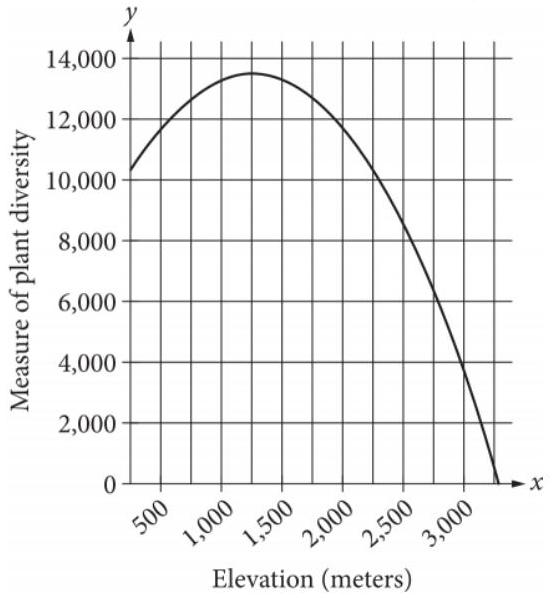
\includegraphics[max width=\textwidth]{2025_06_15_5ccb8dd1752fe76599e7g-082}
\end{center}

The quadratic function graphed above models a particular measure of plant diversity as a function of the elevation in a region of Switzerland. According to the model, which of the following is closest to the elevation, in meters, at which plant diversity is greatest?\\
A. 13,500\\
B. 3,000\\
C. 1,250\\
D. 250

Square P has a side length of $x$ inches. Square Q has a perimeter that is 176 inches greater than the perimeter of square P . The function $f$ gives the area of square Q , in square inches. Which of the following defines $f$ ?\\
A. $f(x)=(x+44)^{2}$\\
B. $f(x)=(x+176)^{2}$\\
C. $f(x)=(176 x+44)^{2}$\\
D. $f(x)=(176 x+176)^{2}$

The surface area of a cube is $6\left(\frac{a}{4}\right)^{2}$, where $a$ is a positive constant. Which of the following gives the perimeter of one face of the cube?\\
A. $\frac{a}{4}$\\
B. $a$\\
C. $4 a$\\
D. $6 a$

\section*{ID: a26c29f7}
The function $f$ is defined by $f(x)=7 x^{3}$. In the $x y$-plane, the graph of $y=g(x)$ is the result of shifting the graph of $y=f(x)$ down 2 units. Which equation defines function $g$ ?\\
A. $g(x)=\frac{7}{2} x^{3}$\\
B. $g(x)=7 x^{\frac{3}{2}}$\\
C. $g(x)=7 x^{3}+2$\\
D. $g(x)=7 x^{3}-2$

\section*{ID: e1391dd6}
According to Moore's law, the number of transistors included on microprocessors doubles every 2 years. In 1985, a microprocessor was introduced that had 275,000 transistors. Based on this information, in which of the following years does Moore's law estimate the number of transistors to reach 1.1 million?\\
A. 1987\\
B. 1989\\
C. 1991\\
D. 1994

The function $f$ is defined by $f(x)=270(0.1)^{x}$. What is the value of $f(0)$ ?\\
A. 0\\
B. 1\\
C. 27\\
D. 270

The function $g$ is defined by $g(x)=x^{2}+9$. For which value of $x$ is $g(x)=25$ ?\\
A. 4\\
B. 5\\
C. 9\\
D. 13

\section*{ID: d46da42c}
$$
f(x)=x^{2}+4
$$

The function $f$ is defined as shown. Which of the following graphs in the $x y$ plane could be the graph of $y=f(x)$ ?\\
A.\\
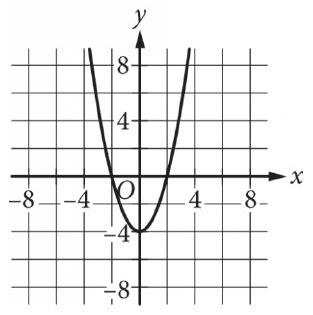
\includegraphics[max width=\textwidth, center]{2025_06_15_5ccb8dd1752fe76599e7g-089(3)}\\
B.\\
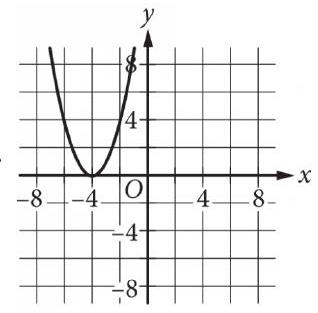
\includegraphics[max width=\textwidth, center]{2025_06_15_5ccb8dd1752fe76599e7g-089(1)}\\
C.\\
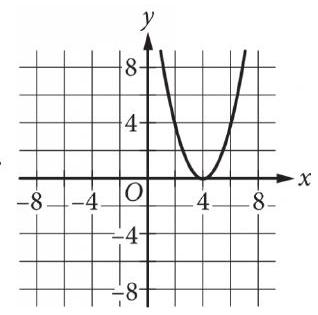
\includegraphics[max width=\textwidth, center]{2025_06_15_5ccb8dd1752fe76599e7g-089}\\
D.\\
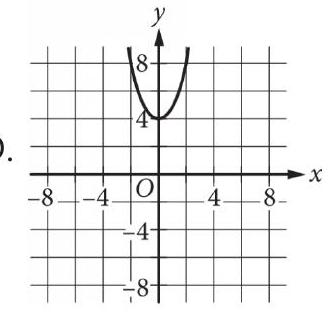
\includegraphics[max width=\textwidth, center]{2025_06_15_5ccb8dd1752fe76599e7g-089(2)}

\section*{ID: 4209aefe}
The function $f(x)=206(1.034)^{x}$ models the value, in dollars, of a certain bank account by the end of each year from 1957 through 1972, where $x$ is the number of years after 1957 . Which of the following is the best interpretation of " $f(5)$ is approximately equal to $243^{\prime \prime}$ in this context?\\
A. The value of the bank account is estimated to be approximately 5 dollars greater in 1962 than in 1957.\\
B. The value of the bank account is estimated to be approximately 243 dollars in 1962 .\\
C. The value, in dollars, of the bank account is estimated to be approximately 5 times greater in 1962 than in 1957.\\
D. The value of the bank account is estimated to increase by approximately 243 dollars every 5 years between 1957 and 1972.

\section*{ID: 5bf0f84a}
$$
h(t)=-16 t^{2}+110 t+72
$$

The function above models the height $h$, in feet, of an object above ground $t$ seconds after being launched straight up in the air. What does the number 72 represent in the function?\\
A. The initial height, in feet, of the object\\
B. The maximum height, in feet, of the object\\
C. The initial speed, in feet per second, of the object\\
D. The maximum speed, in feet per second, of the object

\section*{ID: c048055c}
A model predicts that the population of Springfield was 15,000 in 2005. The model also predicts that each year for the next 5 years, the population $p$ increased by $4 \%$ of the previous year's population. Which equation best represents this model, where $x$ is the number of years after 2005 , for $x \leq 5$ ?\\
A. $p=0.96$ msup\\
B. $p=1.04 \mathrm{msup}$\\
C. $p=15,000 \mathrm{msup}$\\
D. $p=15,000 \mathrm{msup}$

\section*{ID: 70ebd3d0}
$$
N(d)=115(0.90)^{d}
$$

The function $N$ defined above can be used to model the number of species of brachiopods at various ocean depths $d$, where $d$ is in hundreds of meters. Which of the following does the model predict?\\
A. For every increase in depth by 1 meter, the number of brachiopod species decreases by 115 .\\
B. For every increase in depth by 1 meter, the number of brachiopod species decreases by $10 \%$.\\
C. For every increase in depth by 100 meters, the number of brachiopod species decreases by 115 .\\
D. For every increase in depth by 100 meters, the number of brachiopod species decreases by $10 \%$.

\section*{ID: de39858a}
The function $h$ is defined by $h(x)=a^{x}+b$, where $a$ and $b$ are positive constants. The graph of $y=h(x)$ in the $x y$-plane passes through the points $(0,10)$ and $\left(-2, \frac{325}{36}\right)$. What is the value of $a b$ ?\\
A. $\frac{1}{4}$\\
B. $\frac{1}{2}$\\
C. 54\\
D. 60

\begin{center}
\begin{tabular}{|c|c|}
\hline
$x$ & $y$ \\
\hline
21 & -8 \\
\hline
23 & 8 \\
\hline
25 & -8 \\
\hline
\end{tabular}
\end{center}

The table shows three values of $x$ and their corresponding values of $y$, where $y=f(x)+4$ and $f$ is a quadratic function. What is the $y$-coordinate of the $y$-intercept of the graph of $y=f(x)$ in the $x y$-plane?

$$
g(x)=11\left(\frac{1}{12}\right)^{x}
$$

If the given function $g$ is graphed in the $x y$-plane, where $y=g(x)$, what is the $y$-intercept of the graph?\\
A. $(0,11)$\\
B. $(0,132)$\\
C. $(0,1)$\\
D. $(0,12)$

\section*{ID: 97158b3a}
The area $A$, in square centimeters, of a rectangular painting can be represented by the expression $w(w+29)$, where $w$ is the width, in centimeters, of the painting. Which expression represents the length, in centimeters, of the painting?\\
A. $w$\\
B. 29\\
C. $(w+29)$\\
D. $w(w+29)$

\section*{ID: 84e8cc72}
A quadratic function models the height, in feet, of an object above the ground in terms of the time, in seconds, after the object is launched off an elevated surface. The model indicates the object has an initial height of 10 feet above the ground and reaches its maximum height of 1,034 feet above the ground 8 seconds after being launched. Based on the model, what is the height, in feet, of the object above the ground 10 seconds after being launched?\\
A. 234\\
B. 778\\
C. 970\\
D. 1,014

\section*{ID: d8ace155}
A company opens an account with an initial balance of $\$ 36,100.00$. The account earns interest, and no additional deposits or withdrawals are made. The account balance is given by an exponential function $A$, where $A(t)$ is the account balance, in dollars, $t$ years after the account is opened. The account balance after 13 years is $\$ 68,071.93$. Which equation could define $A$ ?\\
A. $A(t)=36,100.00(1.05)^{t}$\\
B. $A(t)=31,971.93(1.05)^{t}$\\
C. $A(t)=31,971.93(0.05)^{t}$\\
D. $A(t)=36,100.00(0.05)^{t}$

\section*{ID: dba7432e}
\begin{center}
\begin{tabular}{|c|c|}
\hline
$x$ & $f(x)$ \\
\hline
0 & 5 \\
\hline
1 & $\frac{5}{2}$ \\
\hline
2 & $\frac{5}{4}$ \\
\hline
3 & $\frac{5}{8}$ \\
\hline
\end{tabular}
\end{center}

The table above gives the values of the function $f$ for some values of $x$. Which of the following equations could define $f$ ?\\
A. $f(x)=5\left(2^{x+1}\right)$\\
B. $f(x)=5\left(2^{x}\right)$\\
C. $f(x)=5\left(2^{-(x+1)}\right)$\\
D. $f(x)=5\left(2^{-x}\right)$

Function $f$ is defined by $f(x)=(x+6)(x+5)(x+1)$. Function $g$ is defined by $g(x)=f(x-1)$. The graph of $y=g(x)$ in the $x y$-plane has $x$-intercepts at $(a, 0),(b, 0)$, and $(c, 0)$, where $a, b$, and $c$ are distinct constants. What is the value of $a+b+c$ ?\\
A. -15\\
B. -9\\
C. 11\\
D. 15

\section*{ID: f1c81b3b}
The exponential function $g$ is defined by $g(x)=19 \cdot a^{x}$, where $a$ is a positive constant. If $g(3)=2,375$, what is the value of $g(4)$ ?

\section*{ID: 4b642eef}
The total distance $d$, in meters, traveled by an object moving in a straight line can be modeled by a quadratic function that is defined in terms of $t$, where $t$ is the time in seconds. At a time of 10.0 seconds, the total distance traveled by the object is 50.0 meters, and at a time of 20.0 seconds, the total distance traveled by the object is 200.0 meters. If the object was at a distance of 0 meters when $t=0$, then what is the total distance traveled, in meters, by the object after 30.0 seconds?

\section*{ID: 0aaef7aa}
The function $p$ is defined by $p(n)=7 n^{3}$. What is the value of $n$ when $p(n)$ is equal to 56 ?\\
A. 2\\
B. $\frac{8}{3}$\\
C. 7\\
D. 8

\section*{ID: b7cd6ca6}
The equation $E(t)=5(1.8)^{t}$ gives the estimated number of employees at a restaurant, where $t$ is the number of years since the restaurant opened. Which of the following is the best interpretation of the number 5 in this context?\\
A. The estimated number of employees when the restaurant opened\\
B. The increase in the estimated number of employees each year\\
C. The number of years the restaurant has been open\\
D. The percent increase in the estimated number of employees each year

$$
f(x)=4 x^{2}-50 x+126
$$

The given equation defines the function $f$. For what value of $x$ does $f(x)$ reach its minimum?

\section*{ID: 9f2ecade}
$$
h(x)=x^{3}+a x^{2}+b x+c
$$

The function $h$ is defined above, where $a, b$, and $c$ are integer constants. If the zeros of the function are $-5,6$, and 7 , what is the value of $c$ ?

The function $f$ is defined by $f(x)=8 \sqrt{x}$. For what value of $x$ does $f(x)=48$ ?\\
A. 6\\
B. 8\\
C. 36\\
D. 64

\section*{ID: 0e61101e}
The function $f$ is defined by the given equation. If $g(x)=f(x+2)$, which of the following equations defines the function $g$ ?\\
A. $g(x)=18(4)^{x}$\\
B. $g(x)=144(4)^{x}$\\
C. $g(x)=18(8)^{x}$\\
D. $g(x)=81(16)^{x}$

$$
f(x)=(x+7)^{2}+4
$$

The function $f$ is defined by the given equation. For what value of $x$ does $f(x)$ reach its minimum?

The function $f$ is defined by $f(x)=x^{3}+15$. What is the value of $f(2)$ ?\\
A. 20\\
B. 21\\
C. 23\\
D. 24

Kao measured the temperature of a cup of hot chocolate placed in a room with a constant temperature of 70 degrees Fahrenheit ( ${ }^{\circ} \mathrm{F}$ ). The temperature of the hot chocolate was $185^{\circ} \mathrm{F}$ at 6:00 p.m. when it started cooling. The temperature of the hot chocolate was $156^{\circ} \mathrm{F}$ at 6:05 p.m. and $135^{\circ} \mathrm{F}$ at 6:10 p.m. The hot chocolate's temperature continued to decrease. Of the following functions, which best models the temperature $T(m)$, in degrees Fahrenheit, of Kao's hot chocolate $m$ minutes after it started cooling?\\
A. $T(m)=185(1.25)^{m}$\\
B. $T(m)=185(0.85)^{m}$\\
C. $T(m)=(185-70)(0.75)^{\frac{m}{5}}$\\
$T(m)=70+115(0.75)^{\frac{m}{5}}$\\
D.

\section*{ID: 50418728}
\begin{center}
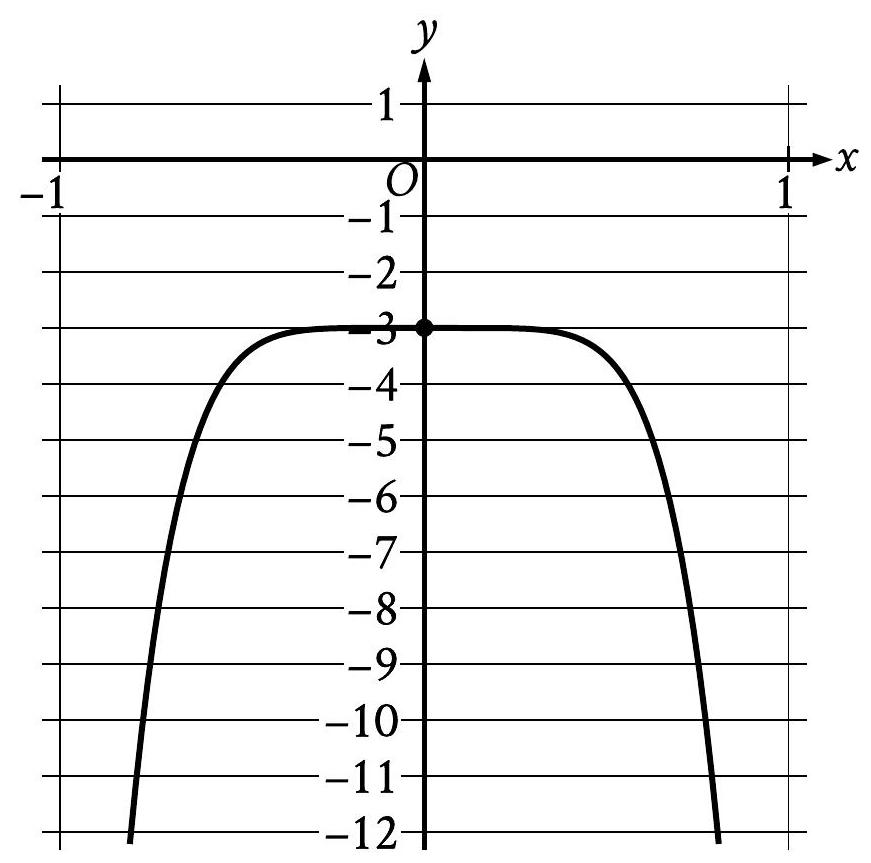
\includegraphics[max width=\textwidth]{2025_06_15_5ccb8dd1752fe76599e7g-113}
\end{center}

The graph of the polynomial function $f$, where $y=f(x)$, is shown. The $y$-intercept of the graph is $(0, y)$. What is the value of $y$ ?

\section*{ID: f5e8ccf1}
$$
f(x)=(x+4)(x-1)(2 x-3)
$$

The function $f$ is defined above. Which of the following is NOT an $x$-intercept of the graph of the function in the $x y$-plane?\\
A. $(-4,0)$\\
B. $\left(-\frac{2}{3}, 0\right)$\\
C. $(1,0)$\\
D. $\left(\frac{3}{2}, 0\right)$

\section*{ID: 1fe10d97}
$$
p(t)=90,000(1.06)^{t}
$$

The given function $p$ models the population of Lowell $t$ years after a census. Which of the following functions best models the population of Lowell $m$ months after the census?\\
A. $r(m)=\frac{90,000}{12}(1.06)^{m}$\\
B. $r(m)=90,000\left(\frac{1.06}{12}\right)^{m}$\\
C. $r(m)=90,000\left(\frac{1.06}{12}\right)^{\frac{m}{12}}$\\
D. $r(m)=90,000(1.06)^{\frac{m}{12}}$

\section*{ID: b73ee6cf}
The population of a town is currently 50,000 , and the population is estimated to increase each year by $3 \%$ from the previous year. Which of the following equations can be used to estimate the number of years, $t$, it will take for the population of the town to reach 60,000 ?\\
A. $50,000=60,000(0.03)^{t}$\\
B. $50,000=60,000(3)^{t}$\\
c. $60,000=50,000(0.03)^{t}$\\
D. $60,000=50,000(1.03)^{t}$

\section*{ID: 08d03fe4}
For the exponential function $f$, the value of $f(1)$ is $k$, where $k$ is a constant. Which of the following equivalent forms of the function $f$ shows the value of $k$ as the coefficient or the base?\\
A. $f(x)=50(2)^{x+1}$\\
B. $f(x)=80(2)^{x}$\\
C. $f(x)=128(2)^{x-1}$\\
D. $f(x)=205(2)^{x-2}$

\section*{ID: 3918e8bc}
An object is kicked from a platform. The equation $h=-4.9 t^{2}+7 t+9$ represents this situation, where $h$ is the height of the object above the ground, in meters, $t$ seconds after it is kicked. Which number represents the height, in meters, from which the object was kicked?\\
A. 0\\
B. 4.9\\
C. 7\\
D. 9

\section*{ID: 7eed640d}
$$
h(x)=-16 x^{2}+100 x+10
$$

The quadratic function above models the height above the ground $h$, in feet, of a projectile $x$ seconds after it had been launched vertically. If $y=h(x)$ is graphed in the $x y$-plane, which of the following represents the real-life meaning of the positive $x$-intercept of the graph?\\
A. The initial height of the projectile\\
B. The maximum height of the projectile\\
C. The time at which the projectile reaches its maximum height\\
D. The time at which the projectile hits the ground

The function $f$ is defined by $f(x)=5 x^{2}$. What is the value of $f(8)$ ?\\
A. 40\\
B. 50\\
C. 80\\
D. 320

\begin{center}
\begin{tabular}{|c|c|}
\hline
$x$ & $f(x)$ \\
\hline
1 & $a$ \\
\hline
2 & $a^{5}$ \\
\hline
3 & $a^{9}$ \\
\hline
\end{tabular}
\end{center}

For the exponential function $f$, the table above shows several values of $x$ and their corresponding values of $f(x)$, where $a$ is a constant greater than 1 . If $k$ is a constant and $f(k)=a^{29}$, what is the value of $k$ ?

\section*{ID: 044c1cb7}
$$
h(x)=x^{2}-3
$$

Which table gives three values of $x$ and their corresponding values of $h(x)$ for the given function $h$ ?\\
A.

\begin{center}
\begin{tabular}{|c|c|c|c|}
\hline
$x$ & 1 & 2 & 3 \\
\hline
$h(x)$ & 4 & 5 & 6 \\
\hline
\end{tabular}
\end{center}

B.

\begin{center}
\begin{tabular}{|c|c|c|c|}
\hline
$x$ & 1 & 2 & 3 \\
\hline
$h(x)$ & -2 & 1 & 6 \\
\hline
\end{tabular}
\end{center}

c.

\begin{center}
\begin{tabular}{|c|c|c|c|}
\hline
$x$ & 1 & 2 & 3 \\
\hline
$h(x)$ & -1 & 1 & 3 \\
\hline
\end{tabular}
\end{center}

D.

\begin{center}
\begin{tabular}{|c|c|c|c|}
\hline
$x$ & 1 & 2 & 3 \\
\hline
$h(x)$ & -2 & 1 & 3 \\
\hline
\end{tabular}
\end{center}

Bacteria are growing in a liquid growth medium. There were 300,000 cells per milliliter during an initial observation. The number of cells per milliliter doubles every 3 hours. How many cells per milliliter will there be 15 hours after the initial observation?\\
A. $1,500,000$\\
B. $2,400,000$\\
C. $4,500,000$\\
D. $9,600,000$

\section*{ID: 4d037075}
\begin{center}
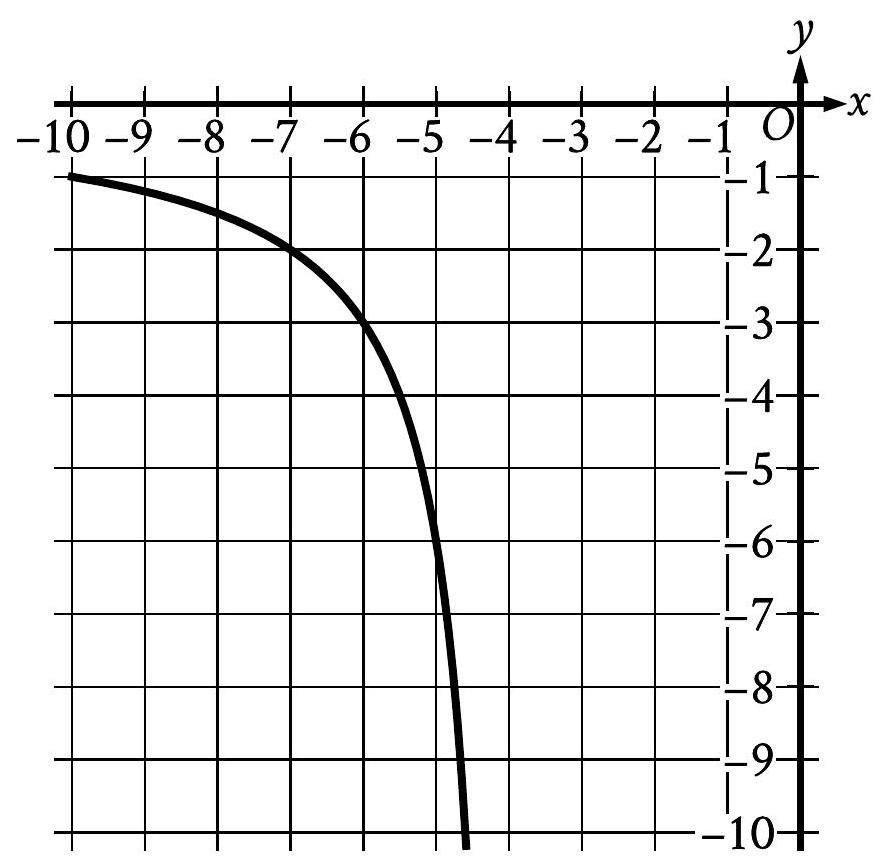
\includegraphics[max width=\textwidth]{2025_06_15_5ccb8dd1752fe76599e7g-124}
\end{center}

The rational function $f$ is defined by an equation in the form $f(x)=\frac{a}{x+b}$, where $a$ and $b$ are constants. The partial graph of $y=f(x)$ is shown. If $g(x)=f(x+4)$, which equation could define function $g$ ?\\
A. $g(x)=\frac{6}{x}$\\
B. $g(x)=\frac{6}{x+4}$\\
C. $g(x)=\frac{6}{x+8}$\\
D. $g(x)=\frac{6(x+4)}{x+4}$

$$
f(x)=(x-10)(x+13)
$$

The function $f$ is defined by the given equation. For what value of $x$ does $f(x)$ reach its minimum?\\
A. -130\\
B. -13\\
C. $-\frac{23}{2}$\\
D. $-\frac{3}{2}$

The area $A$, in square centimeters, of a rectangular cutting board can be represented by the expression $w(w+9)$, where $w$ is the width, in centimeters, of the cutting board. Which expression represents the length, in centimeters, of the cutting board?\\
A. $w(w+9)$\\
B. $w$\\
C. 9\\
D. $(w+9)$

\section*{ID: 1853bb35}
For the function $q$, the value of $q(x)$ decreases by $45 \%$ for every increase in the value of $x$ by 1 . If $q(0)=14$, which equation defines $q$ ?\\
A. $q(x)=0.55(14)^{x}$\\
B. $q(x)=1.45(14)^{x}$\\
C. $q(x)=14(0.55)^{x}$\\
D. $q(x)=14(1.45)^{x}$

\section*{ID: a8ae0d22}
Two variables, $x$ and $y$, are related such that for each increase of 1 in the value of $x$, the value of $y$ increases by a factor of 4 . When $x=0, y=200$. Which equation represents this relationship?\\
A. $y=4 \mathrm{msup}$\\
B. $y=4 \mathrm{msup}$\\
C. $y=200 \mathrm{msup}$\\
D. $y=200 \mathrm{msup}$

$$
f(x)=\frac{a-19}{x}+5
$$

In the given function $f, a$ is a constant. The graph of function $f$ in the $x y$-plane, where $y=f(x)$, is translated 3 units down and 4 units to the right to produce the graph of $y=g(x)$. Which equation defines function $g$ ?\\
A. $g(x)=\frac{a-19}{x+4}+2$\\
B. $g(x)=\frac{a-19}{x-4}+2$\\
C. $g(x)=\frac{a-22}{x+4}+5$\\
D. $g(x)=\frac{a-22}{x-4}+5$

\section*{ID: a7711fe8}
What is the minimum value of the function $f$\\
defined by $f(x)=(x-2)^{2}-4$ ?\\
A. -4\\
B. -2\\
C. 2\\
D. 4

Let the function $p$ be defined as $p(x)=\frac{(x-c)^{2}+160}{2 c}$, where $c$ is a constant. If $p(c)=10$, what is the value of $p(12)$ ?\\
A. 10.00\\
B. 10.25\\
C. 10.75\\
D. 11.00

\section*{ID: ee05c84e}
$$
f(x)=(x+0.25 x)(50-x)
$$

The function $f$ is defined above. What is the value of $f(20)$ ?\\
A. 250\\
B. 500\\
C. 750\\
D. 2,000

\section*{ID: 5c00c2c1}
There were no jackrabbits in Australia before 1788 when 24 jackrabbits were introduced. By 1920 the population of jackrabbits had reached 10 billion. If the population had grown exponentially, this would correspond to a $16.2 \%$ increase, on average, in the population each year. Which of the following functions best models the population $p(t)$ of jackrabbits $t$ years after 1788 ?\\
A. $p(t)=1.162(24)^{t}$\\
B. $p(t)=24(2)^{1.162 t}$\\
c. $p(t)=24(1.162)^{t}$\\
D. $p(t)=(24, \cdot 1.162)^{t}$


